\chapter{Image Arithmetic}
\label{ch:lesson02}

Since an image is a 2D array of numbers (Chapter~\ref{ch:lesson01}), basic arithmetic can edit it: add a constant to brighten, subtract to darken, blend two images by weighted averaging, and so on. This chapter highlights an important subtlety: when images are stored as 8-bit unsigned integers, \emph{how} you do the arithmetic matters.

\section{Brightening: add a constant}

A pixel's value represents the amount of light, so adding a positive constant to every pixel should brighten the whole image.

\begin{lstlisting}
img = np.zeros((150, 150), dtype=np.uint8)
cv2.circle(img, (75, 75), 50, 180, -1)
brightened_naive = img + np.uint8(80)
\end{lstlisting}

The result (Figure~\ref{fig:l02-1}) is not what was intended.

\begin{figure}[h]
\centering
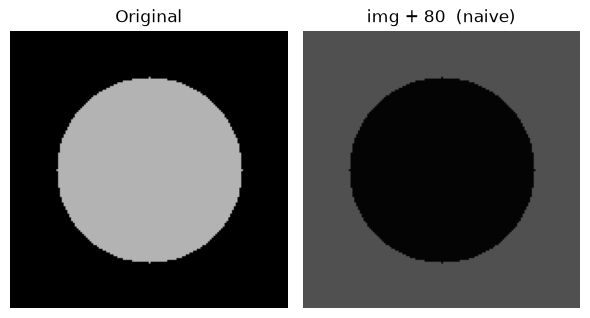
\includegraphics[width=0.55\textwidth]{figures/lesson02_fig01.png}
\caption{Look closely at the circle: it became \emph{darker}, not brighter.}
\label{fig:l02-1}
\end{figure}

\subsection*{The problem: \code{uint8} overflow}

An 8-bit unsigned integer can only represent 0 to 255, so $220+80=300$ does not fit. NumPy's \code{uint8} arithmetic \textbf{wraps around} (like a car odometer rolling over), silently computing $300 \bmod 256 = 44$ instead of \textbf{clamping} at 255 --- the same fixed-width overflow any low-level integer type has, applied silently and with no warning:
\begin{equation}
\texttt{np.array([200, 250, 220], dtype=np.uint8) + np.uint8(80)} \;\longrightarrow\; \texttt{[24, 74, 44]}
\end{equation}

\subsection*{The fix: saturating arithmetic}

OpenCV's arithmetic functions (\code{cv2.add}, \code{cv2.subtract}, \ldots) use \textbf{saturating} arithmetic: results are clamped to the valid range (0--255 for \code{uint8}) rather than wrapping --- almost always what is actually wanted.

\begin{lstlisting}
brightened_saturated = cv2.add(img, 80)
\end{lstlisting}

Figure~\ref{fig:l02-2} compares all three results side by side.

\begin{figure}[h]
\centering
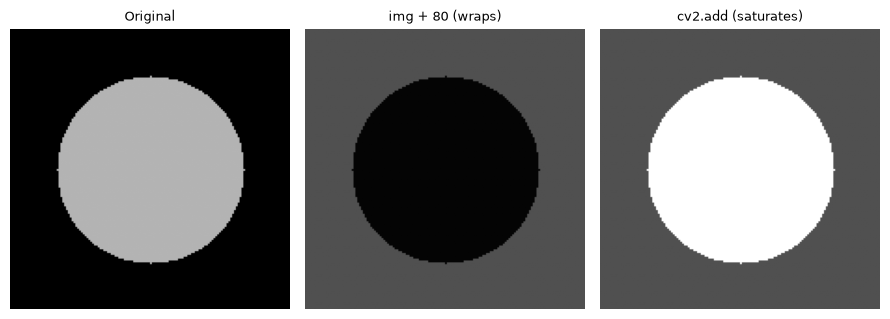
\includegraphics[width=0.9\textwidth]{figures/lesson02_fig02.png}
\caption{Naive NumPy addition wraps (darkens); \code{cv2.add} saturates (clamps at 255) --- the same idea applies at the bottom end for \code{cv2.subtract}, clamped at 0 instead of wrapping to a large positive value.}
\label{fig:l02-2}
\end{figure}

\section{Brightening only part of an image, with a mask}

Often one wants to adjust brightness selectively --- e.g., lighten a foreground subject without touching the background. Given a binary mask (from thresholding or segmentation, Chapters~\ref{ch:lesson03}--\ref{ch:lesson04}), only copy the brightened result where the mask is set.

\begin{lstlisting}
fully_brightened = cv2.add(photo, np.full_like(photo, 60))
result = photo.copy()
result[foreground_mask > 0] = fully_brightened[foreground_mask > 0]
\end{lstlisting}

Figure~\ref{fig:l02-3} shows the photo, the mask, and the result.

\begin{figure}[h]
\centering
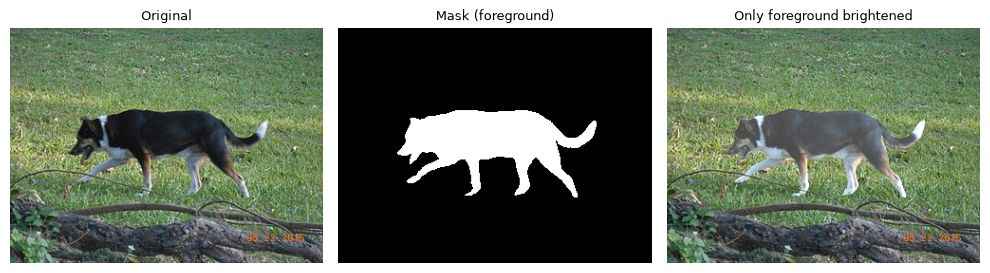
\includegraphics[width=0.85\textwidth]{figures/lesson02_fig03.png}
\caption{Photo, foreground mask, and the selectively brightened result. \attrib{Photo: \href{https://commons.wikimedia.org/wiki/File:Dog_walking_sideview_grass.JPG}{Wikimedia Commons}.}}
\label{fig:l02-3}
\end{figure}

\begin{notebox}
\code{cv2.add} (and several other OpenCV functions) also accept a \code{mask} argument directly, which performs exactly this select-and-copy in one call: \code{cv2.add(photo, 60, mask=foreground\_mask)} --- writing only into the masked region and leaving the rest of the destination untouched.
\end{notebox}

\section{Blending two images}

A weighted sum of two images --- a \textbf{cross-dissolve} --- is the same saturating arithmetic, generalized: \code{cv2.addWeighted(a, alpha, b, beta, gamma)} computes $a\cdot\alpha + b\cdot\beta + \gamma$, saturated, as swept across five values of $\alpha$ in Figure~\ref{fig:l02-4}.

\begin{figure}[h]
\centering
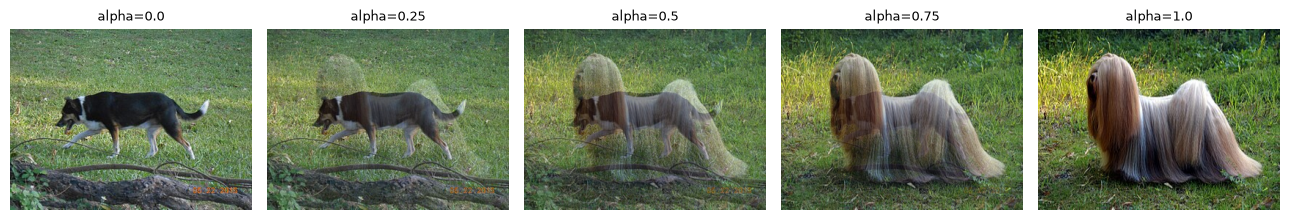
\includegraphics[width=0.95\textwidth]{figures/lesson02_fig04.png}
\caption{\code{cv2.addWeighted} at five values of $\alpha$, cross-dissolving between two dog photos. \attrib{Photos: \href{https://commons.wikimedia.org/wiki/File:Dog_walking_sideview_grass.JPG}{Wikimedia Commons}, \href{https://commons.wikimedia.org/wiki/File:Lhasaapso.jpg}{Wikimedia Commons}.}}
\label{fig:l02-4}
\end{figure}

\section{Difference imaging}

Subtracting two images (with an absolute value, so both directions of change matter equally) highlights exactly what differs between them --- the basis of simple motion/change detection, reused when comparing reconstructions against ground truth in later lessons.

\begin{lstlisting}
difference = cv2.absdiff(before, after)
\end{lstlisting}

Figure~\ref{fig:l02-5} shows the result.

\begin{figure}[h]
\centering
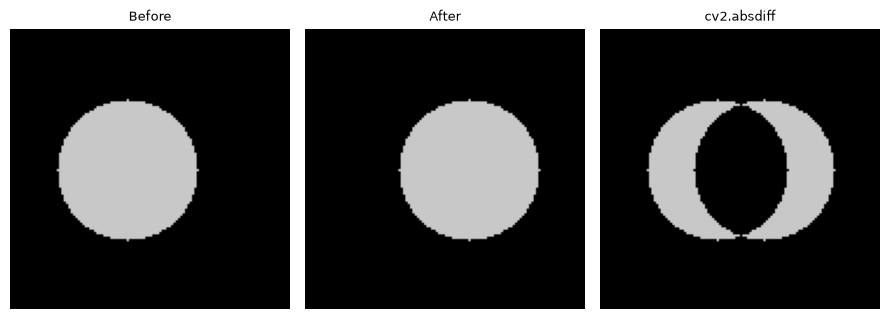
\includegraphics[width=0.85\textwidth]{figures/lesson02_fig05.png}
\caption{The difference image is zero everywhere nothing changed, bright wherever the circle used to be or now is, and dark in the region where it is present in both frames.}
\label{fig:l02-5}
\end{figure}

\subsection*{Exercises}
\begin{enumerate}
  \item Predict, then check, what \code{cv2.subtract(img, 150)} does to a pixel whose value is 100 --- does it wrap around like the naive NumPy addition did, or saturate?
  \item Use \code{cv2.add} with its \code{mask} argument directly (instead of manually copying with boolean indexing) to reproduce the masked-brightening result, and confirm the two approaches give identical output.
  \item \code{cv2.addWeighted} does not require \code{alpha + beta} to sum to 1 (the \code{gamma} term is added on top). Try values that do not sum to 1 and describe the effect.
\end{enumerate}

\vfill
\fullcode{lesson02}{lesson02_image_arithmetic}
